\documentclass[a4paper,12pt]{article}
%\documentclass{Configuration_Files/Template}

%------------------------------------------------------------------------------
%	REQUIRED PACKAGES AND  CONFIGURATIONS
%------------------------------------------------------------------------------

% CONFIGURATIONS
\usepackage{parskip} % For paragraph layout
\usepackage{setspace} % For using single or double spacing
\usepackage{emptypage} % To insert empty pages
\usepackage{multicol} % To write in multiple columns (executive summary)
\setlength\columnsep{15pt} % Column separation in executive summary
\setlength\parindent{0pt} % Indentation
\raggedbottom  

% PACKAGES FOR TITLES
\usepackage{titlesec}
% \titlespacing{\section}{left spacing}{before spacing}{after spacing}
\titlespacing{\section}{0pt}{3.3ex}{2ex}
\titlespacing{\subsection}{0pt}{3.3ex}{1.65ex}
\titlespacing{\subsubsection}{0pt}{3.3ex}{1ex}
\usepackage{color}

% PACKAGES FOR LANGUAGE AND FONT
\usepackage[english]{babel} % The document is in English  
\usepackage[utf8]{inputenc} % UTF8 encoding
\usepackage[T1]{fontenc} % Font encoding
\usepackage[11pt]{moresize} % Big fonts

% PACKAGES FOR IMAGES
\usepackage{graphicx}
\usepackage{transparent} % Enables transparent images
\usepackage{eso-pic} % For the background picture on the title 
\usepackage{rotating}
\usepackage{subfig} % Numbered and caption subfigures using \subfloat.
\usepackage{tikz} % A package for high-quality hand-made figures.
\usetikzlibrary{}
\graphicspath{{./Images/}} % Directory of the images
\usepackage{caption} % Coloured captions
\usepackage{amsthm,thmtools,xcolor} % Coloured "Theorem"
\usepackage{float}

% STANDARD MATH PACKAGES
\usepackage{amsmath}
\usepackage{amsthm}
\usepackage{amssymb}
\usepackage{amsfonts}
\usepackage{bm}
\usepackage[overload]{empheq} % For braced-style systems of equations.
\usepackage{fix-cm} % To override original LaTeX restrictions on sizes

% PACKAGES FOR TABLES
\usepackage{tabularx}
\usepackage{longtable} % Tables that can span several pages
\usepackage{colortbl}

% PACKAGES FOR ALGORITHMS (PSEUDO-CODE)
\usepackage{algorithm}
\usepackage{algorithmic}

% PACKAGES FOR REFERENCES & BIBLIOGRAPHY
\usepackage[colorlinks=true,linkcolor=black,anchorcolor=black,citecolor=black,filecolor=black,menucolor=black,runcolor=black,urlcolor=black]{hyperref} % Adds clickable links at references
\usepackage{cleveref}
\usepackage[square, numbers, sort&compress]{natbib} % Square brackets, citing references with numbers, citations sorted by appearance in the text and compressed
\bibliographystyle{abbrvnat} % You may use a different style adapted to your field

% OTHER PACKAGES
\usepackage{pdfpages} % To include a pdf file
\usepackage{afterpage}
\usepackage{lipsum} % DUMMY PACKAGE
\usepackage{fancyhdr} % For the headers
\fancyhf{}

%----------------------------------------------------------------------------
%	NEW COMMANDS DEFINED
%----------------------------------------------------------------------------

% EXAMPLES OF NEW COMMANDS
\newcommand{\bea}{\begin{eqnarray}} % Shortcut for equation arrays
\newcommand{\eea}{\end{eqnarray}}
\newcommand{\e}[1]{\times 10^{#1}}  % Powers of 10 notation

%----------------------------------------------------------------------------
%	ADD YOUR PACKAGES (be careful of package interaction)
%----------------------------------------------------------------------------

\usepackage{geometry}
\usepackage{tabularx}
\usepackage{booktabs,xltabular}

%----------------------------------------------------------------------------
%	ADD YOUR DEFINITIONS AND COMMANDS (be careful of existing commands)
%----------------------------------------------------------------------------

% Set uniform margins
\geometry{
  left=0.8in,
  right=0.8in,
  top=1in,
  bottom=1in,
  includehead,
  includefoot
}

\begin{document}
\title{Students\&Companies Design Document} % Title Page
\author{Alessandro Salvatore, Erdal Yalçın, Leonardo Ratti}
\date{Academic Year: 2024-25}
\maketitle


\newpage
\tableofcontents
\section{Introduction}
\subsection{Purpose}
This document contains the design description of the Students\&Company system. It includes
the architectural design, the user interface design and the descrpition of the operations
that the system will perform. It also show how the requirements and use cases detailed
in the RASD document are satisfied by the design of the system. \\ \newline 
This document is intended to be read by the developers of the system, the testers and the
project managers. It is also intended to be used as a reference for the future maintenance
of the system.
\subsection{Scope}
The Students\&Company system is a web application that allows companies to advertise internship opportunities
for university students. A recommendation system is used for enhancing the matching possibilities between the two parties.
The system provides also suggestions for students and companies to increase their chances to get matched by the recommendation system. \\ \newline
A more detailed description of the system can be found in the RASD document, whilist in
this document is provided a detailed description of the design of the system to implement
the requirements and use cases described in the RASD document.
\subsubsection{Definitions}
\subsubsection{Acronyms}
\subsubsection{Abbreviations}
\subsection{Revision History}
\subsection{Reference Documents}
\subsection{Document Structure}

\section{Overall Description}
\subsection{Overview: High-level Components and Interaction}
The following diagram is designed to clearly demonstrate the high-level components required by the system and the relationships between them. 

 The Presentation Layer interacts directly with users and is responsible for managing the front-end side. This layer provides the user interface and collaborates with the Load Balancer and Web Server to optimize system performance and functionality. User interactions within the interface are forwarded from the Presentation Layer to the back-end, enabling additional processing and functionality. Furthermore, to enhance the system’s security and mitigate potential threats from external networks, a Firewall component is incorporated into the architecture. The Business Logic Layer processes incoming requests from the Presentation Layer and facilitates access to the core system functionalities, such as internship applications and recommendation mechanisms, through the use of APIs and Services. In summary, the Business Logic Layer, which houses the Application Server designed in accordance with RESTful standards, ensures the seamless transfer of operations to the Data Layer, thus ensuring the system operates in an efficient, secure, and effective manner.
\begin{figure}[H]
\centering
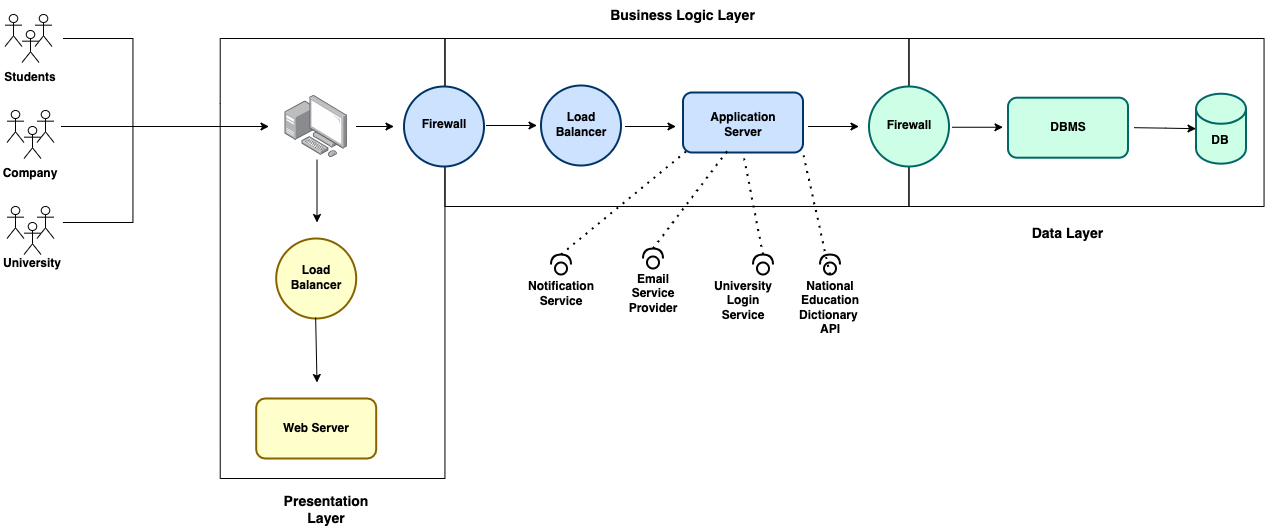
\includegraphics[scale = 0.40]{DD_figures/SingleDiagrams/overviewDiagram.png}
\end{figure}
\subsection{Component View}
In this section we show the components and their relationships. The following
sections will explain the interaction between interfaces and details on each method of interfaces.
\begin{figure}[H]
\centering
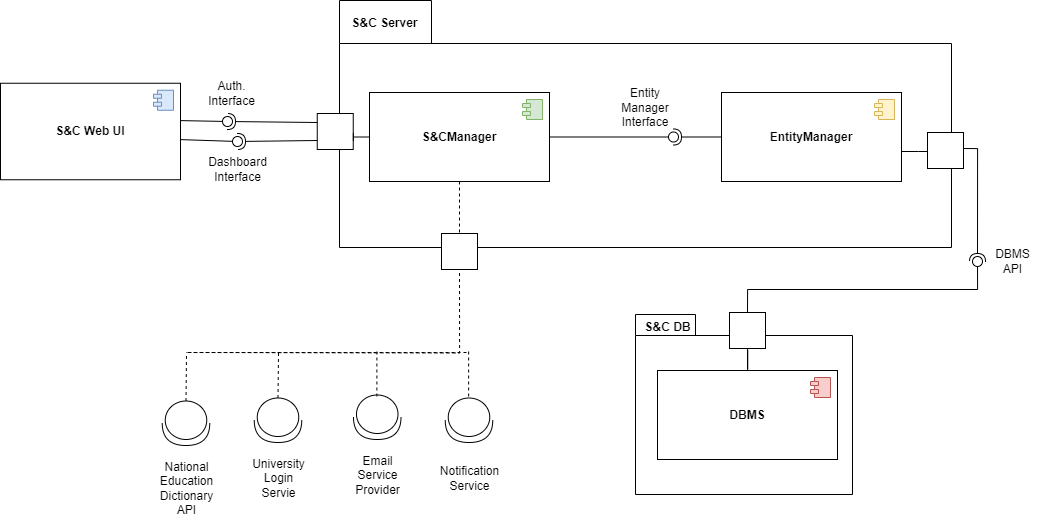
\includegraphics[scale = 0.50]{DD_figures/GeneralComponentDiagram.drawio.png}\\
\caption{Component Diagram of the Student\&Companies System}
\end{figure}

\subsubsection{DB Manager}
This component is responsible for communication with a Database Management System (DBMS).
It follows the Adapter design pattern, allowing other components to interact with the DBMS
without needing to write any SQL code themselves.
\subsubsection{S\&C-SP}
The S\&CSP subsystem implements S\&C's logic. It provides all the system's features, including the recommendation system.
\begin{sidewaysfigure}% Use sidewaysfigure instead of figure
\centering
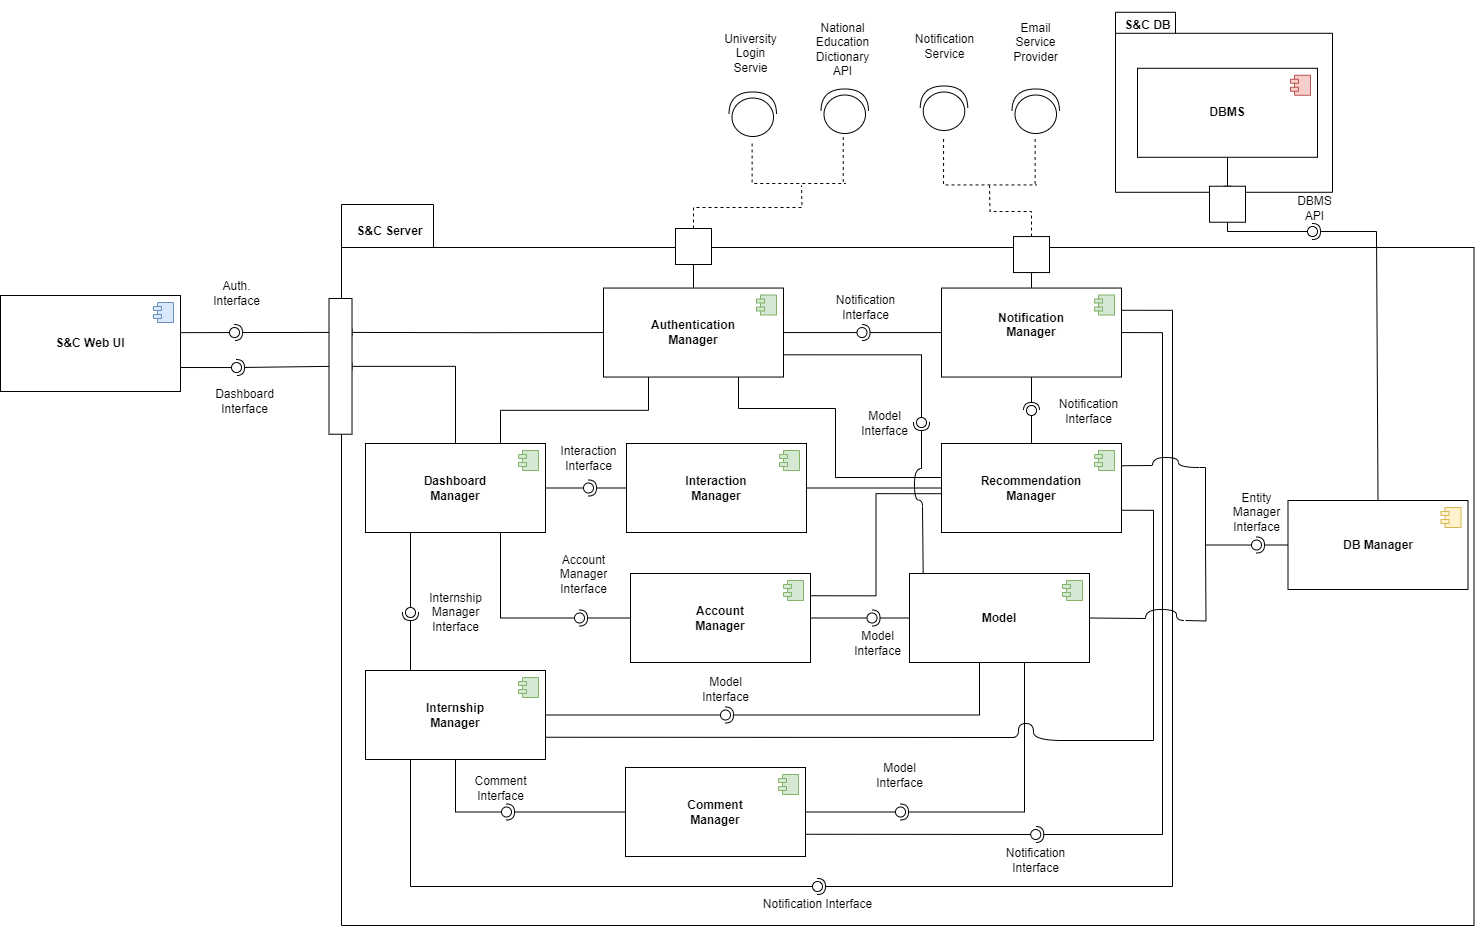
\includegraphics[scale=0.50]{DD_figures/S&C.drawio.png}\\
\caption{Component Diagram of the S\&C-SP subsystem}
\end{sidewaysfigure}
\begin{enumerate}
    \item {Dashboard Manager} :
    \\It's used as an intermediary between the WebUI and the
    other components of the server to provide the web application only the functionality
    strictly necessary for it to work properly.
    \item {Account Manager} :
    \\This component handles the operations needed to manage each User's account, and to view the Users' profiles. It allows Users to login, using the Authentication Manager's interface.
    \item {Authentication Manager} :
    \\This component handles signup, login and logout operations.
    \item {Internship Manager} :
    \\This component handles the operations needed to manage an Internship, to view any information about it and to accept it.
    \item {Comment Manager} :
    \\This component handles the operations needed to view and write comments (complaints and observations.
    \item {Recommendation Manager} :
    \\This component is responsible for the recommendation mechanism for students and internships. It takes the input data from the user interactions with the system and reloads the associated recommendations.
    \item {Interaction Manager} :
    \\This component is responsible for registering feedbacks and interactions of the user with the web application, transforming this information into parameters, and passing it to the recommendation manager for elaboration.
    \item {Notification Manager} :
    \\This component is responsible for the dispatch of notifications.
    \item {Model} :
    \\This component facilitates the interaction with and representation of S\&C-SP data.
\end{enumerate}
\subsection{Deployment View}
We adopted a 3-tier architecture hosted on cloud infrastructure, designed to optimize performance and scalability while reducing costs.

Let's explore more in detail:

\begin{enumerate}
    \item \textbf{Scalability and Flexibility} - the ability to add or remove resources such as virtual machines, performance cores, or memory as needed, in conjunction with the use of load balancing services, allows the servers to adapt to changes in traffic or workload.
    \item \textbf{Security} - Firewalls help to protect the application server against data breaches and other security threats.
    \item \textbf{Cost-efficiency} - the choice of using a cloud provider allows us to only pay for the resources that we are actually using, which can help to lower the overall costs, and in general reduces the waste of resources.
\end{enumerate}

The cloud provider is an ideal choice for hosting large, high-traffic applications. The chosen cloud provider will need to offer all of these features in order to meet our needs.

The web server resides in the De Militarized Zone and is the primary interface for user interaction. The application server executes the core application logic, processing user requests and handling all the operations. Load balancers are implemented to evenly distribute incoming traffic across multiple instances of Web and Application Servers.
\begin{figure}[H]
    \centering
    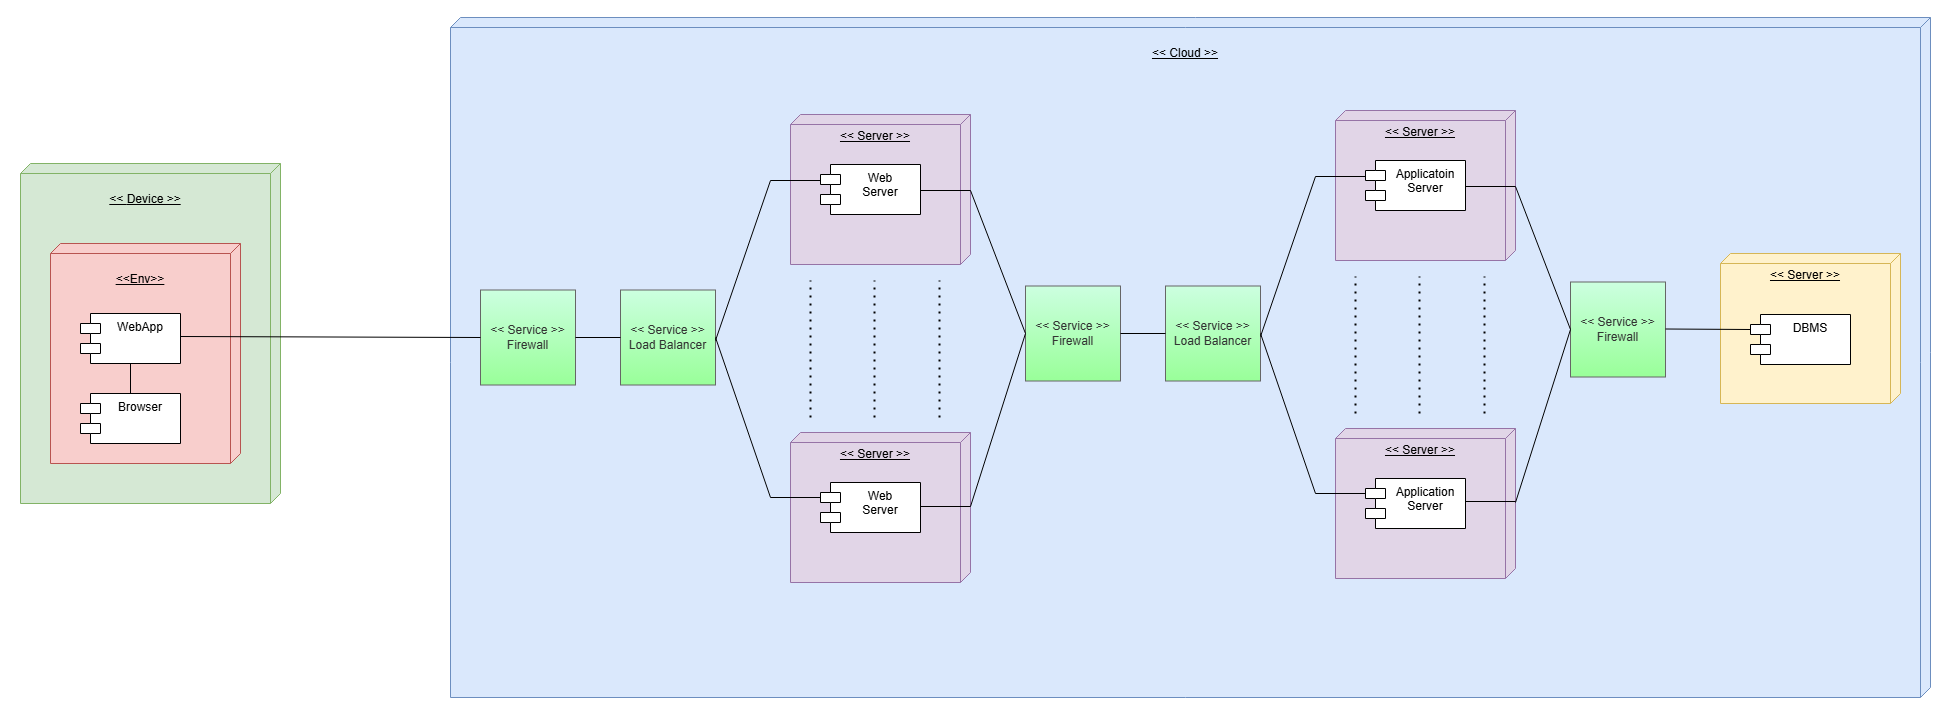
\includegraphics[scale = 0.33]{DD_figures/SingleDiagrams/DeploymentView.png}
    \caption{Component Diagram of the S\&C server subsystem}
    \centering
\end{figure}


\subsection{Runtime View}

\subsubsection*{Student Registers}
The diagram represented below shows the process of a Student creating an account to the S\&C website. First, the Student compiles the sign up form with all the requested information. Immediately after, the University login service, related to the university that the Student inserted in the form, is shown. If the Student logs successfully in its university account then the form information is stored in the DB and a new account is generated. From there, the AuthenticationManager triggers the verification email through the EmailServiceProvider. Eventually, all the companies that advertise an internship that system recognizes valid to recommend are notified of the new student subscription to the platform.
\begin{figure}[H]
\centering
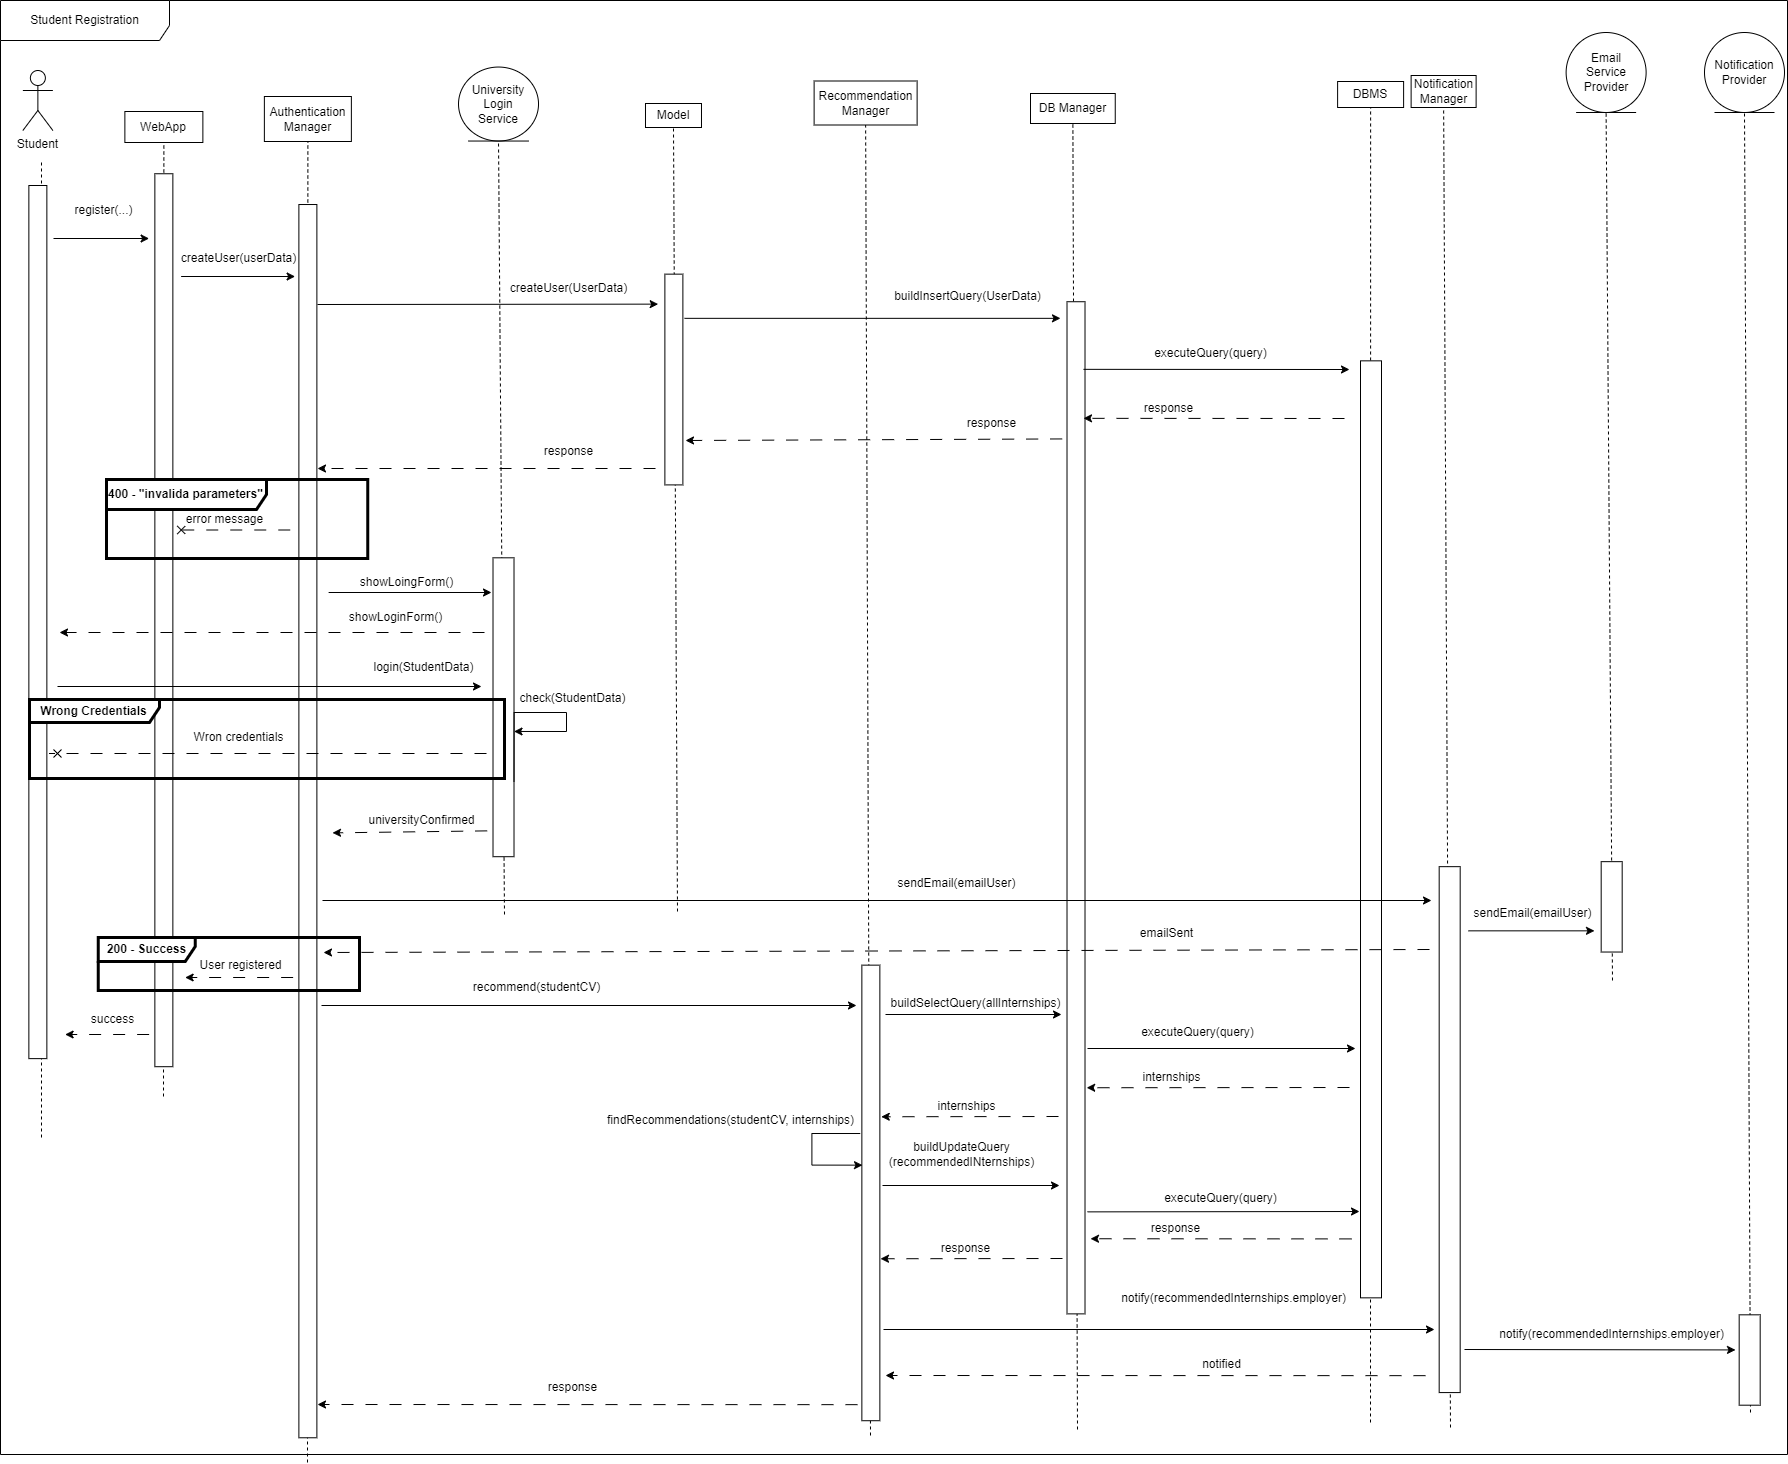
\includegraphics[scale = 0.28]{DD_figures/RuntimeView/StudentRegistrationRV.drawio.png}\\
\caption{Student registers to S\&C}
\end{figure}

\subsubsection*{Company Registers}
The diagram represented down below shows the process of a Company creating an account to the S\&C website. First, the Company compiles the sign up form with all the requested information, then, as the request is submitted through the proper API call, the AuthenticationManager component handles the request, and, if the parameters of the request were valid, the AuthenticationManager
triggers the verification email through the EmailServiceProvider.
\begin{figure}[H]
\centering
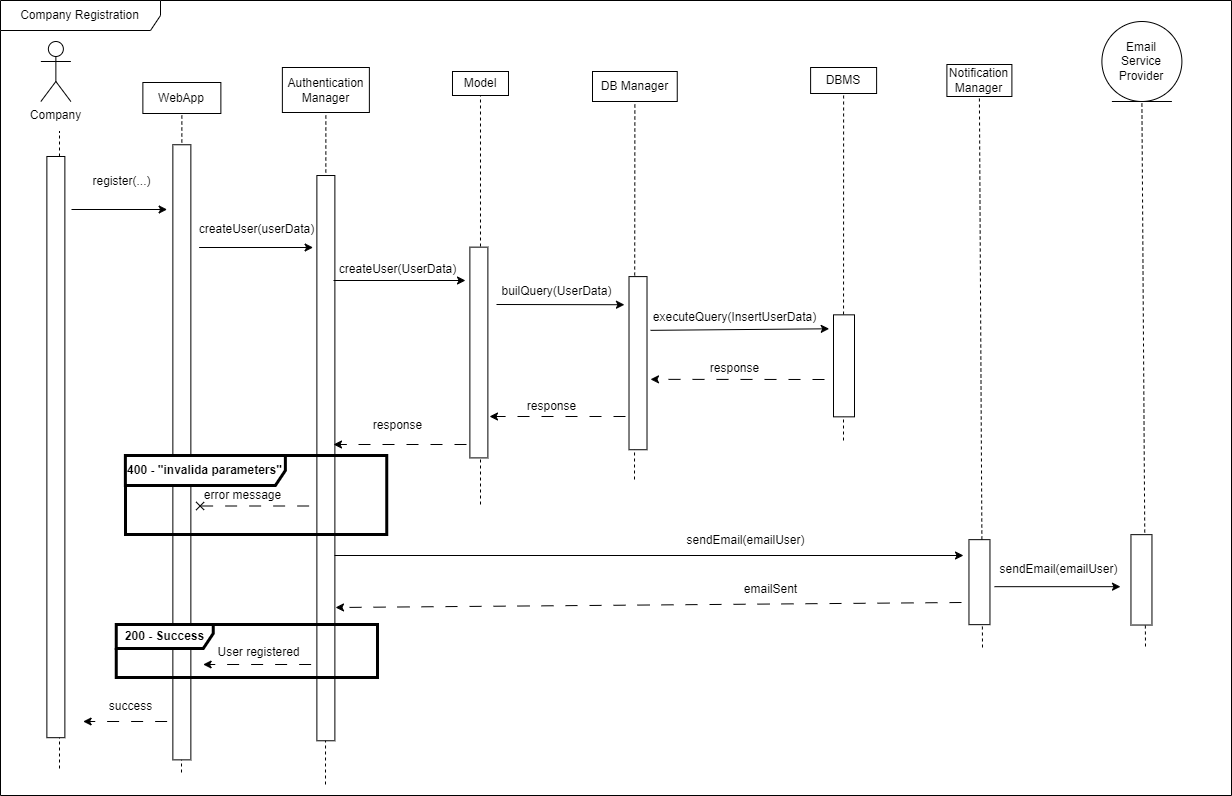
\includegraphics[scale = 0.42]{DD_figures/RuntimeView/CompanyRegistersRV.drawio.png}\\
\caption{Company registers to S\&C}
\end{figure}

\subsubsection*{University Registers}
The diagram represented down below shows the process of a University creating an account to the S\&C website. First, the University compiles the sign up form with all the requested information. From there, the University information is checked using the National Education Dictionary. If the information results correct, then the information is stored in the DB and a new University account is generated. At last, the AuthenticationManager
triggers the verification email through the EmailServiceProvider.
\begin{figure}[H]
\centering
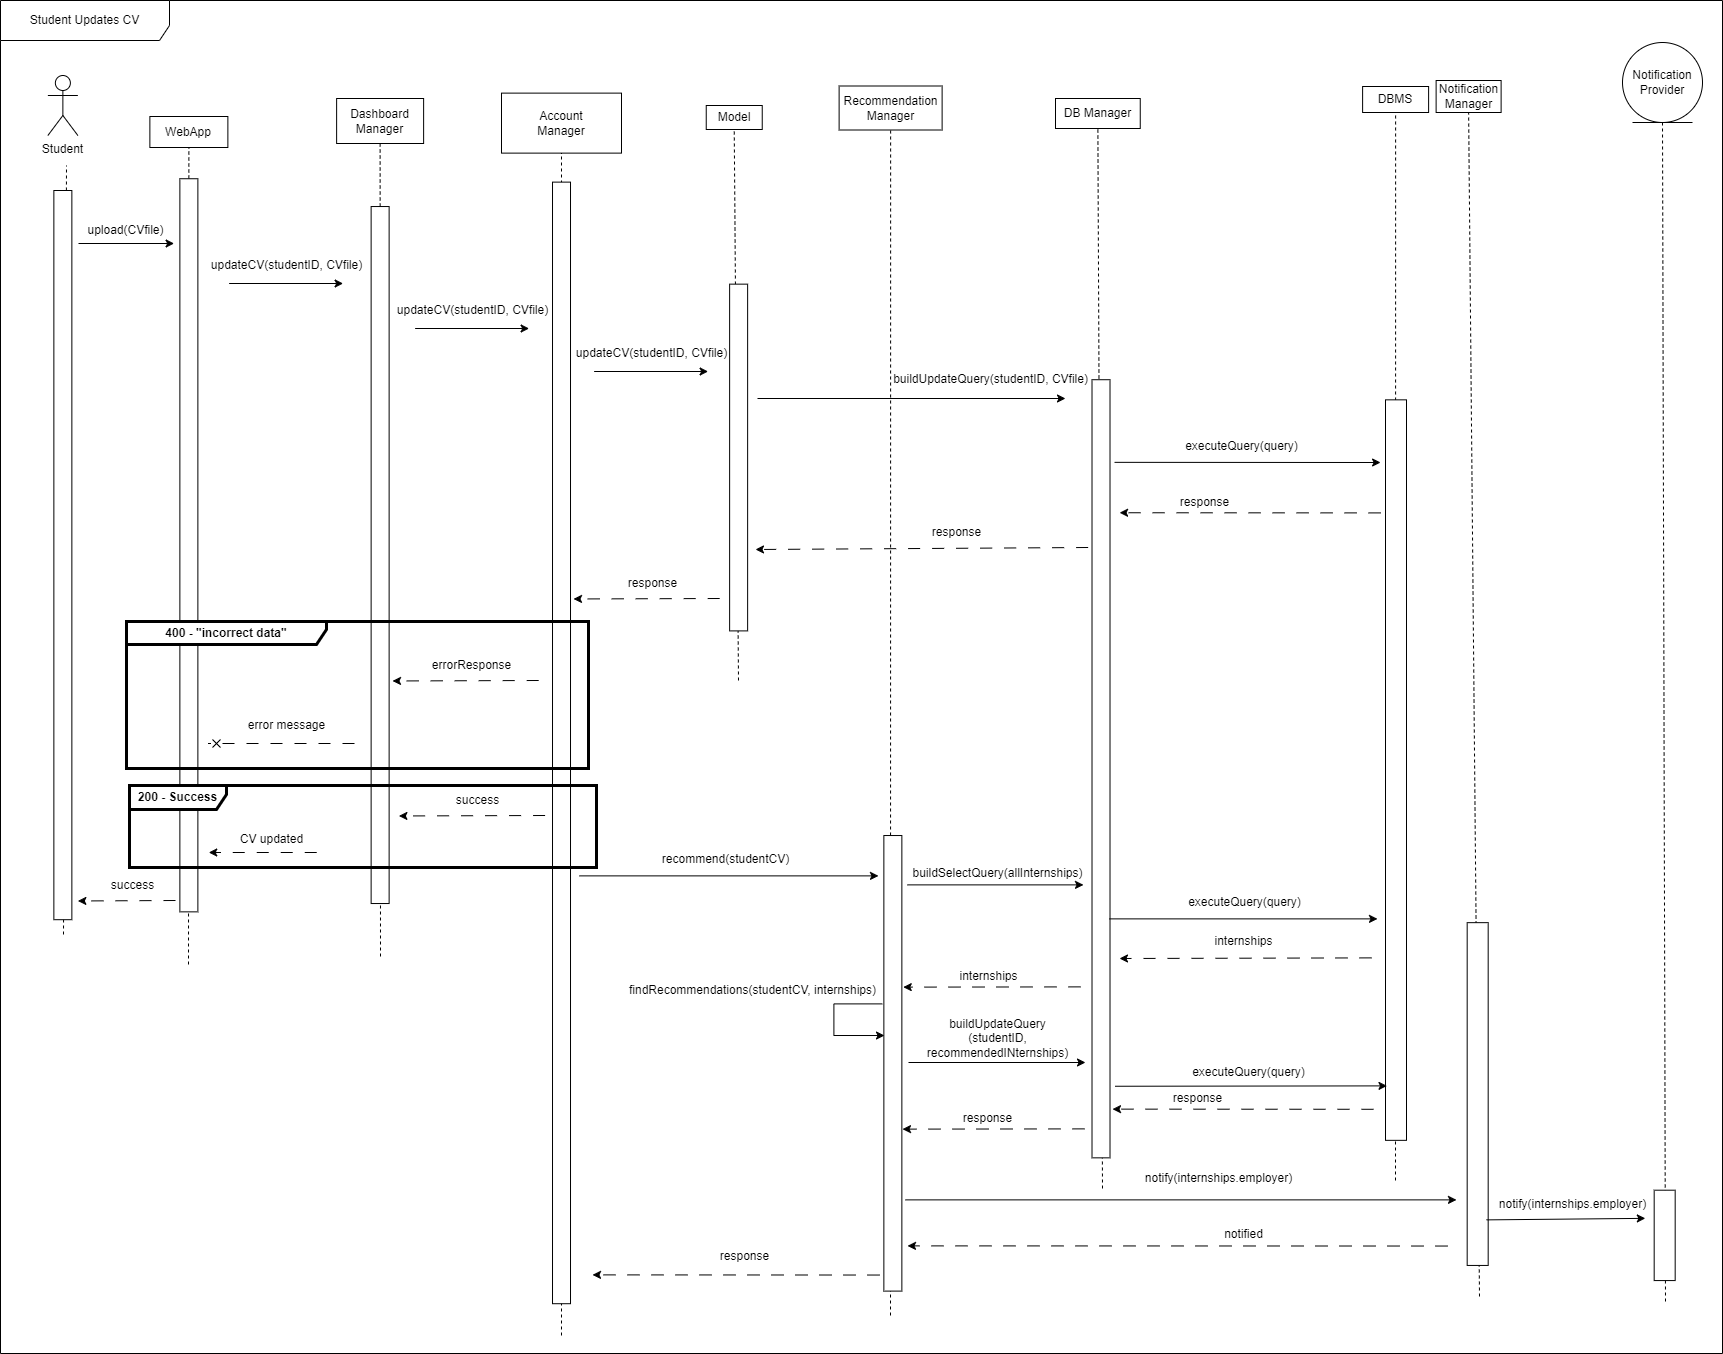
\includegraphics[scale = 0.30]{DD_figures/RuntimeView/StudentUpdatesCV_RV.drawio.png}\\
\caption{university registers to S\&C}
\end{figure}

\subsubsection*{Student Updates CV}
The student initiates the process by uploading their CV, which is handled by the WebApp and subsequently passed to the Dashboard Manager, Account Manager, and Model components for validation and processing. If the data is valid, the CV is updated in the database using a query managed by the DB Manager and DBMS. Upon successful update, the Recommendation Manager generates internship recommendations based on the updated CV, retrieving relevant internships and notifying associated employers. In case of an error (e.g., incorrect data), the system responds with an appropriate error message. Notifications are sent to employers via the Notification Provider, ensuring the flow of updates and recommendations.
\begin{figure}[H]
\centering
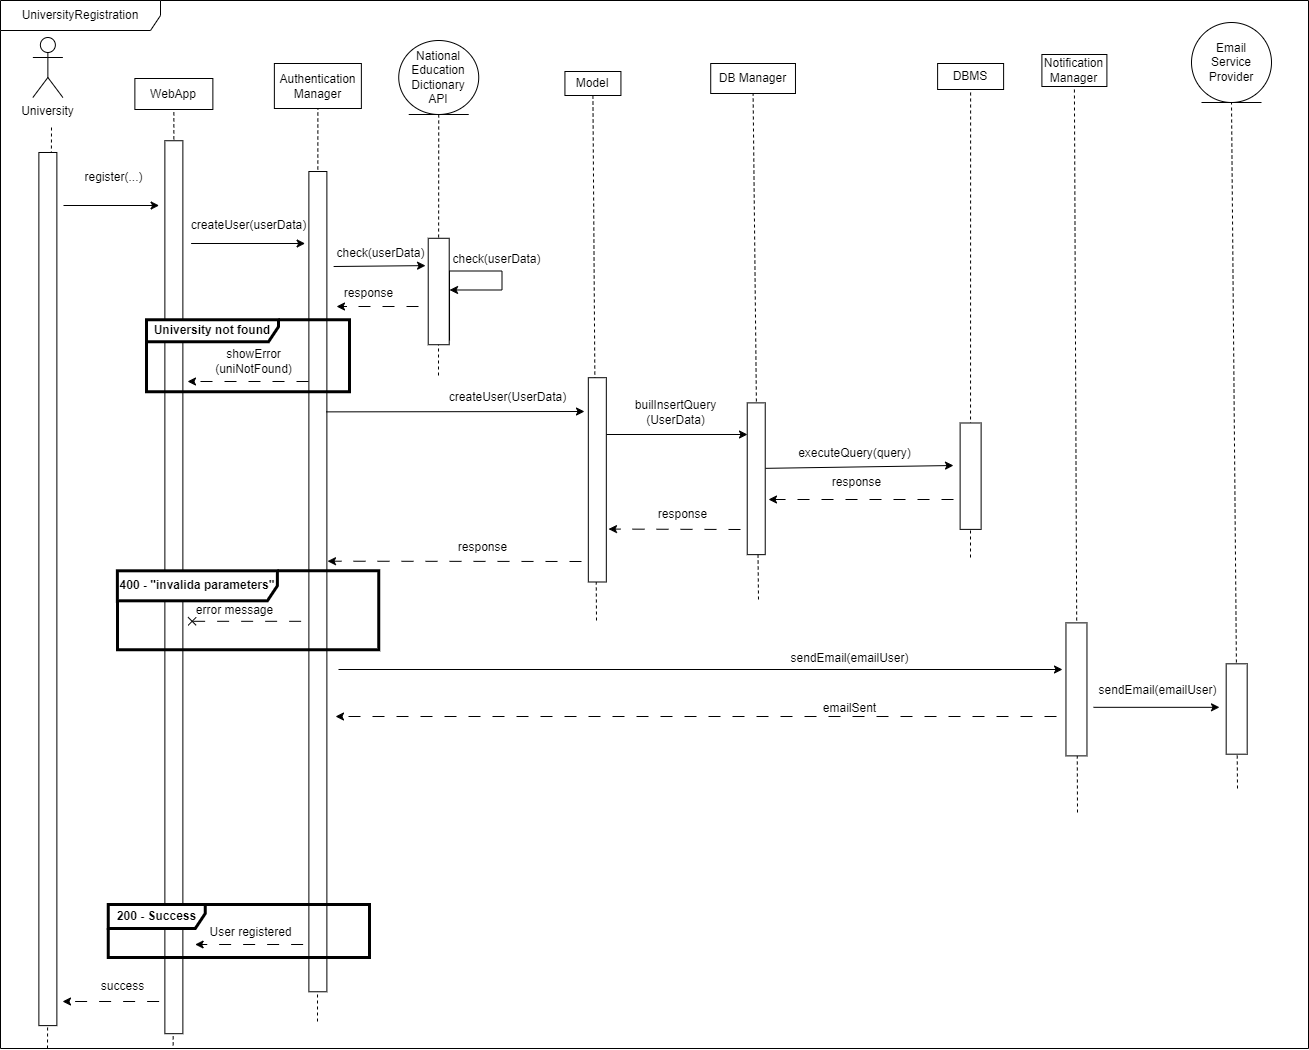
\includegraphics[scale = 0.35]{DD_figures/RuntimeView/UniversityRegistrationRV.drawio.png}\\
\caption{Student Updates CV}
\end{figure}

\subsubsection*{Student changes university}

\begin{figure}[H]
\centering
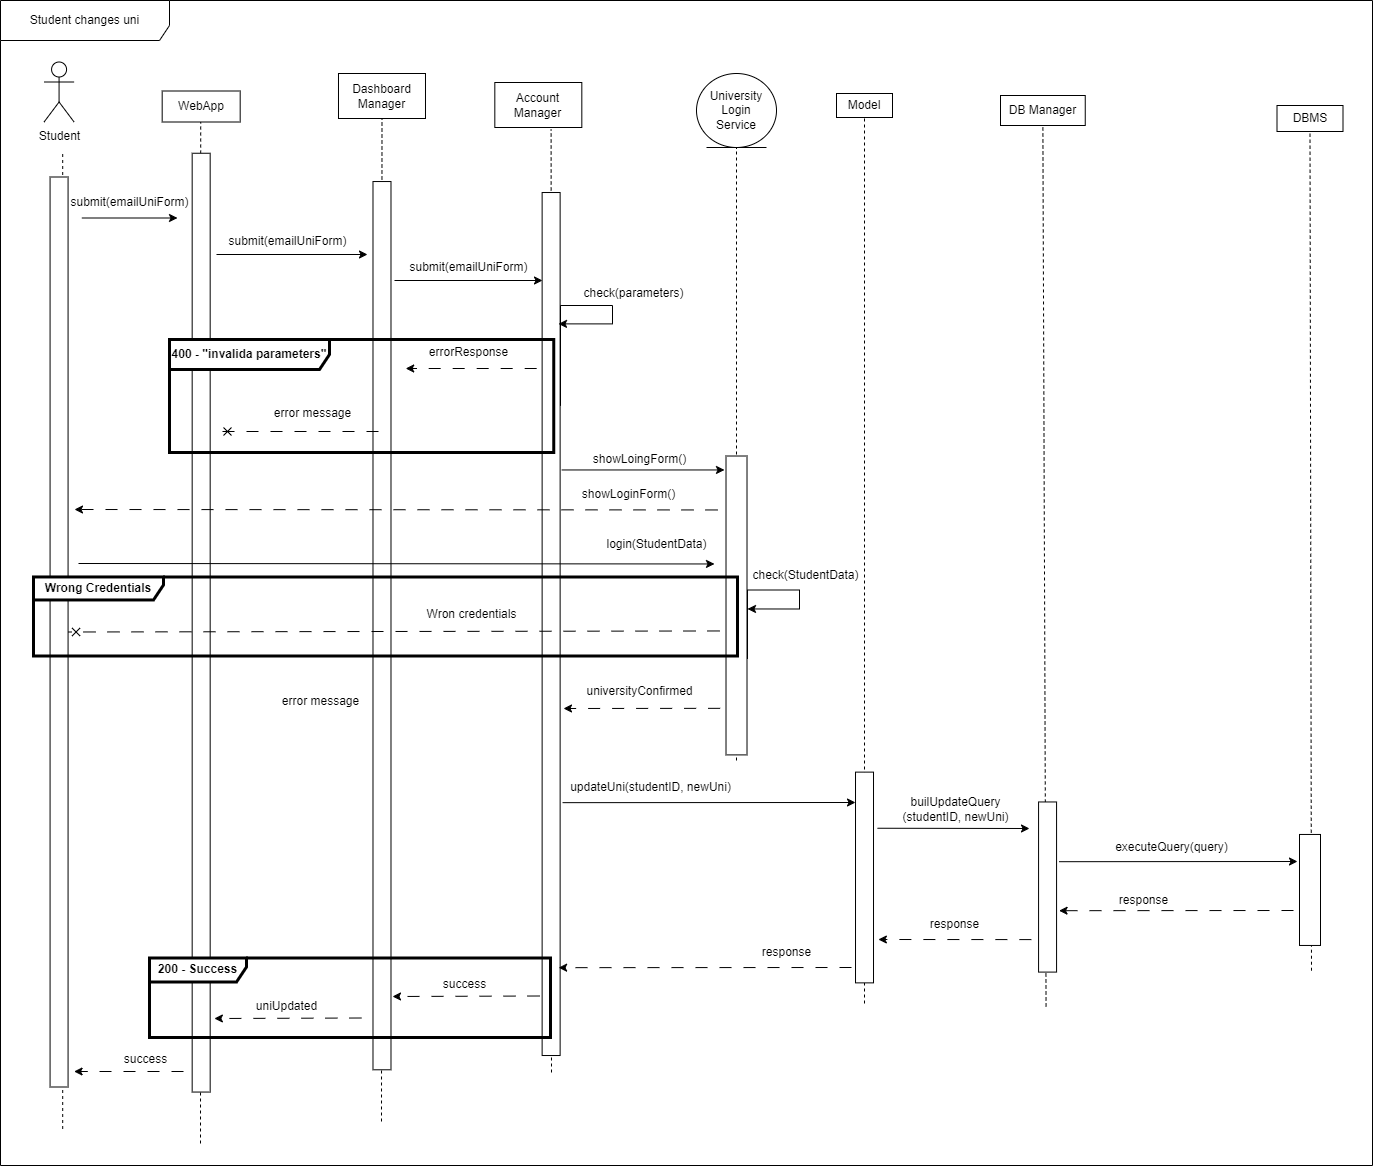
\includegraphics[scale = 0.35]{DD_figures/RuntimeView/StudentChangesUniversityRV.drawio.png}\\
\caption{Student changes university}
\end{figure}

\subsubsection*{Company sends interview form}

\begin{figure}[H]
\centering
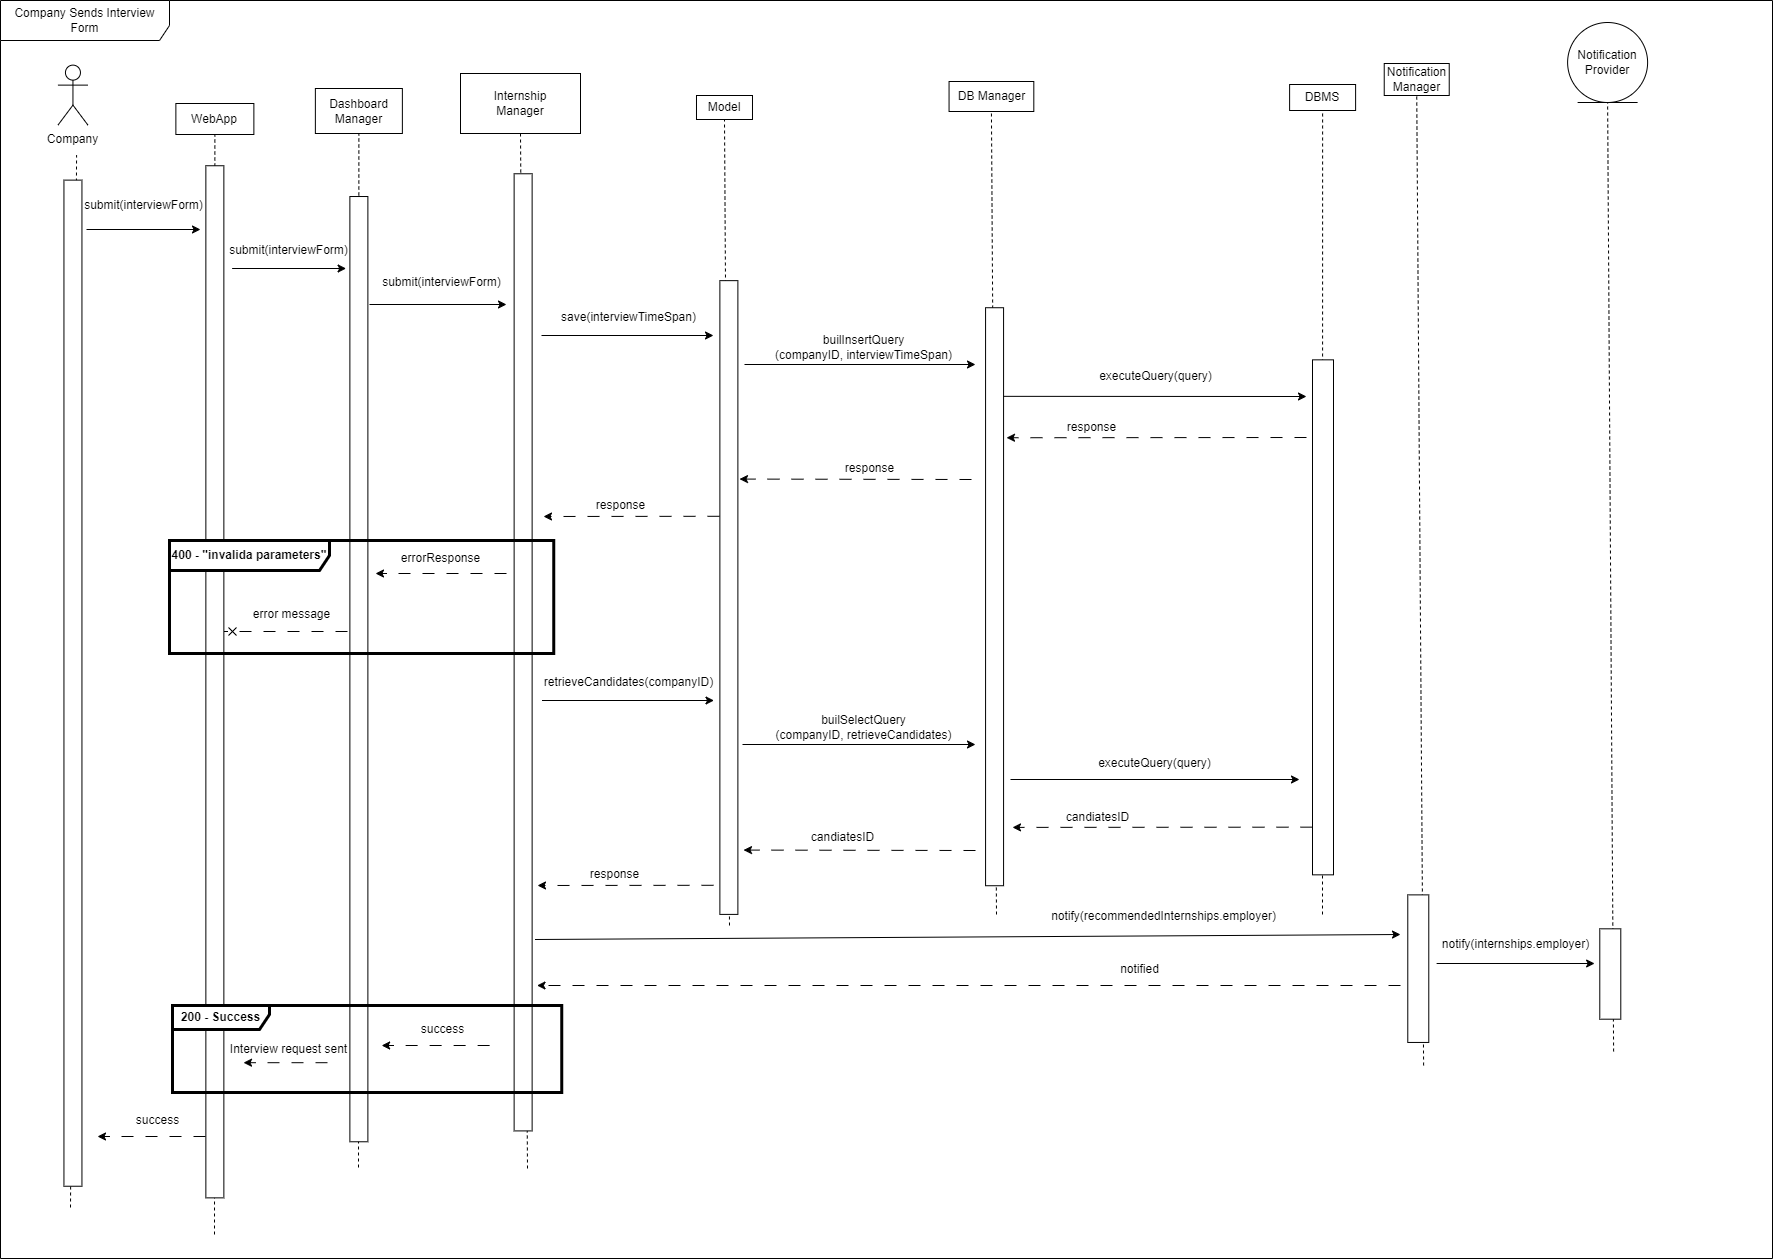
\includegraphics[scale = 0.30]{DD_figures/RuntimeView/CompanySendsInterviewFormRV.drawio.png}\\
\caption{Company sends interview form}
\end{figure}

\subsubsection*{Student selects interview date}

\begin{figure}[H]
\centering
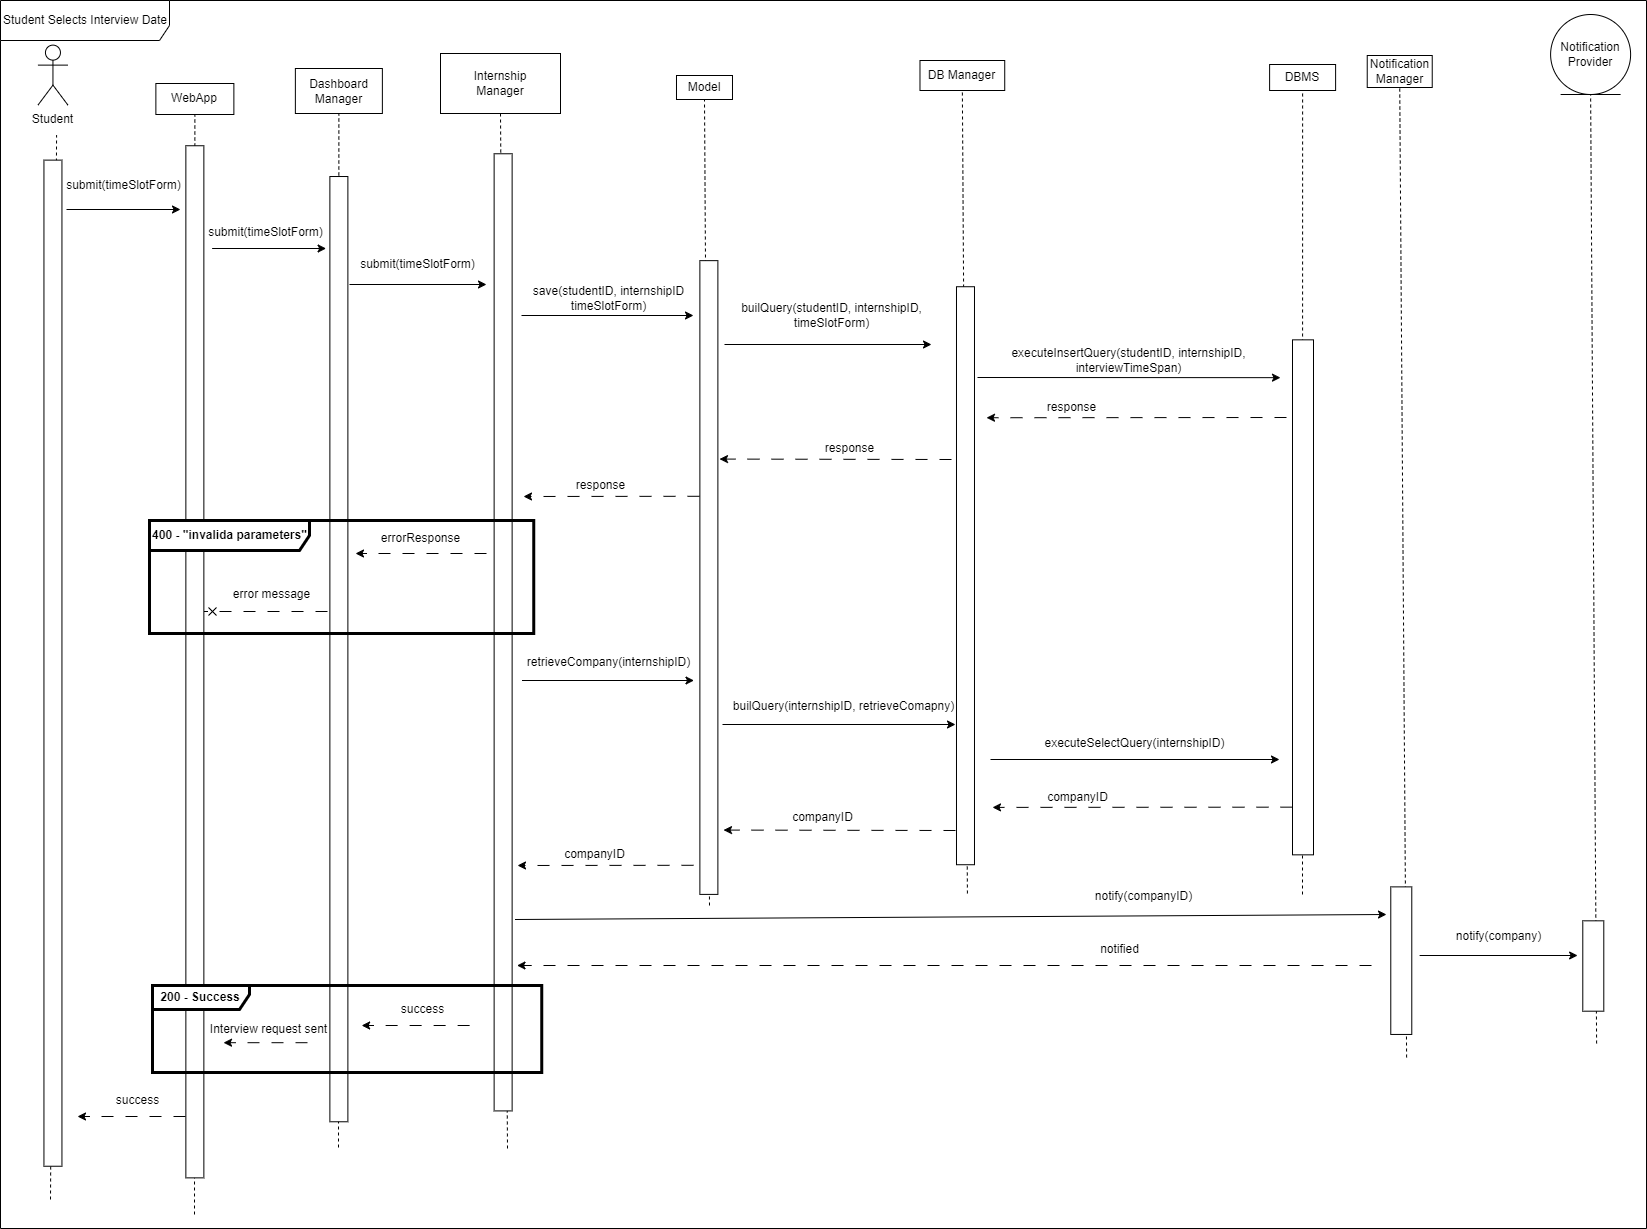
\includegraphics[scale = 0.30]{DD_figures/RuntimeView/StudentSelectsInterviewDateRV.drawio.png}\\
\caption{Student selects interview date}
\end{figure}

\subsubsection*{Company selects candidate}

\begin{figure}[H]
\centering
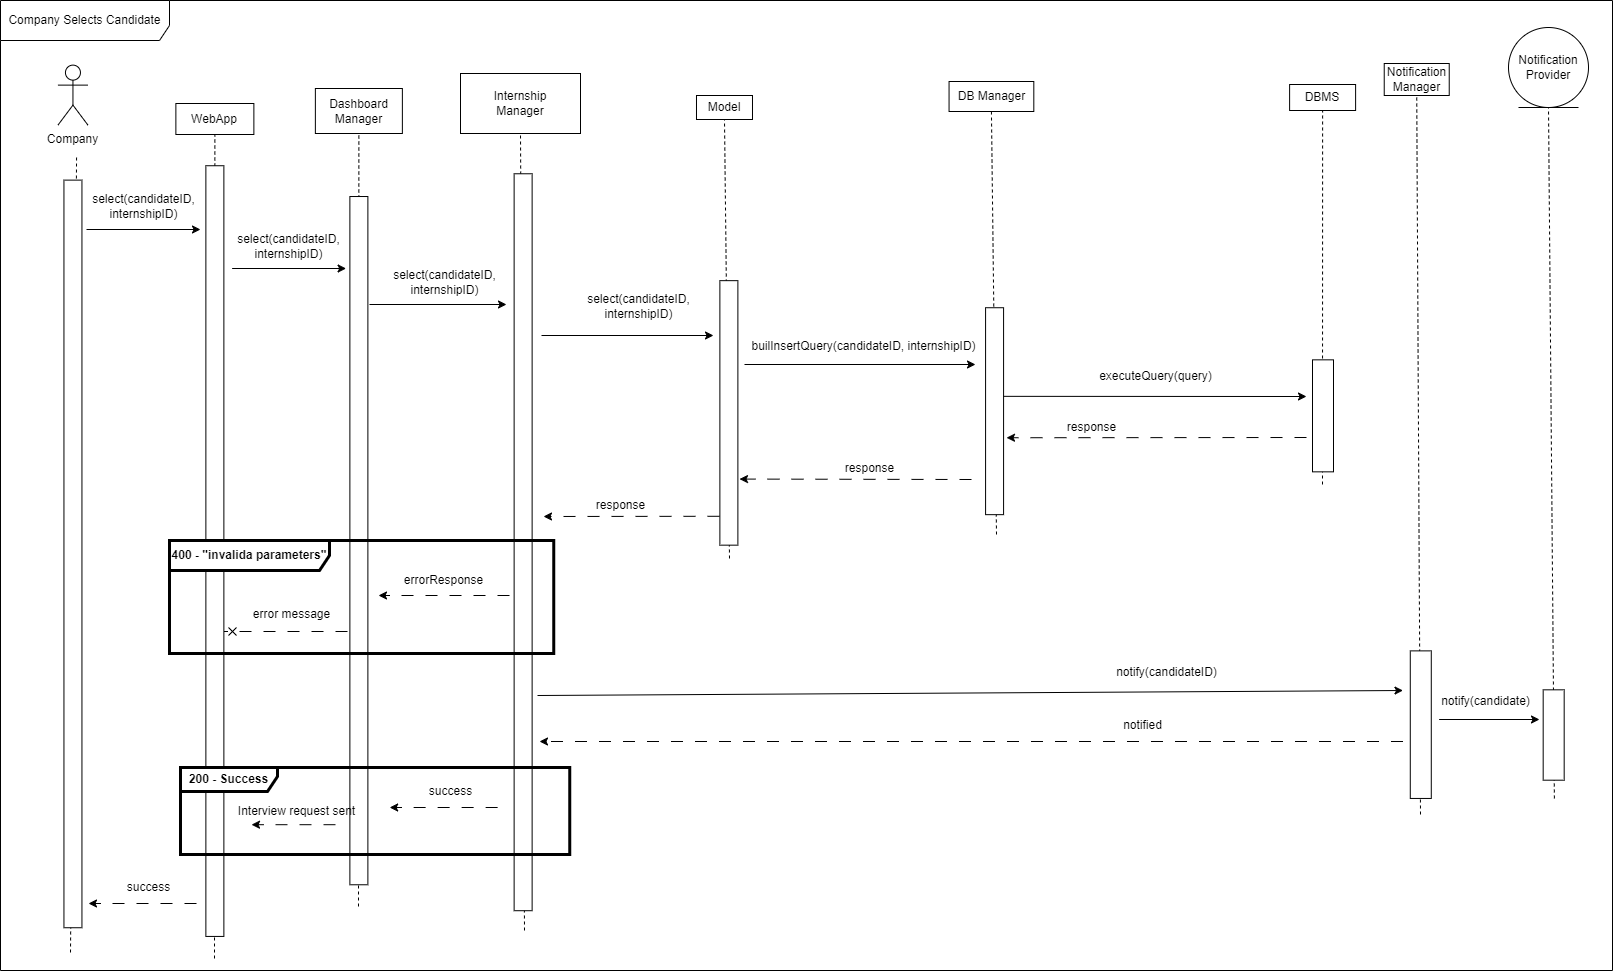
\includegraphics[scale = 0.30]{DD_figures/RuntimeView/CompanySelectsCandidateRV.drawio.png}\\
\caption{Company selects candidate}
\end{figure}


\begin{figure}[H]
    \centering
    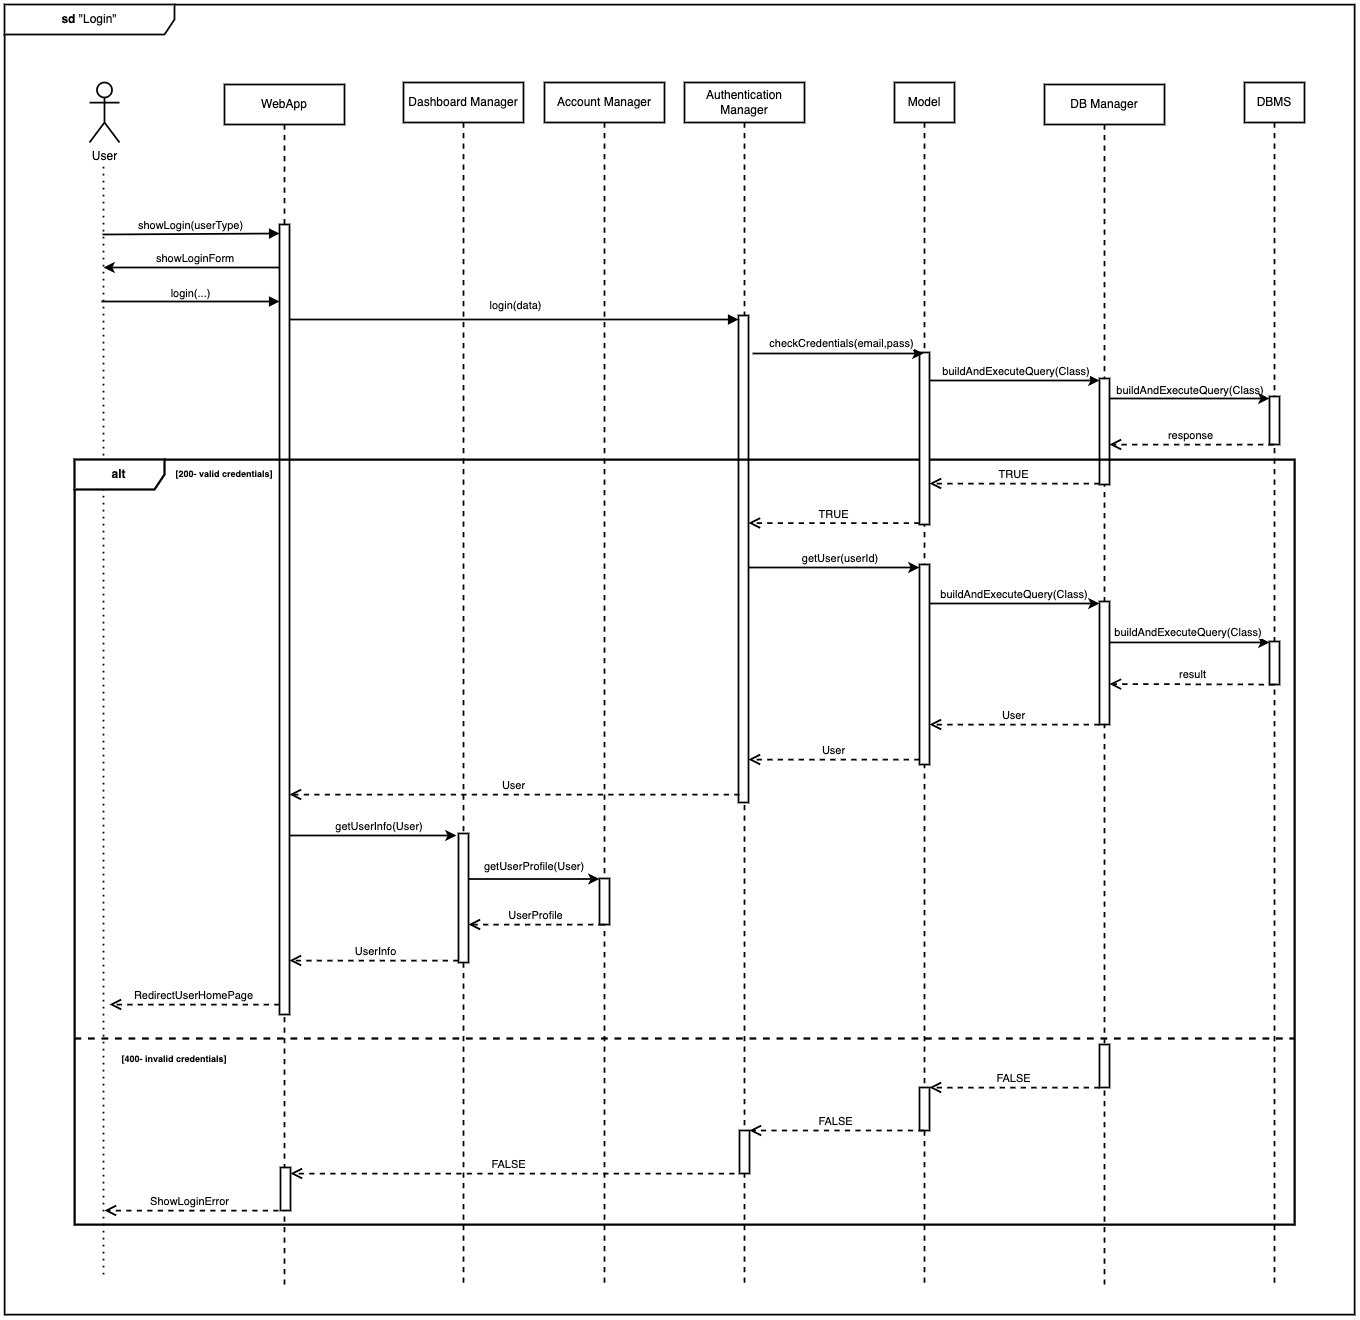
\includegraphics[scale = 0.35]{DD_figures/SingleDiagrams/login.drawio.png}
    \caption{Login}
    \centering
\end{figure}

\begin{figure}[H]
    \centering
    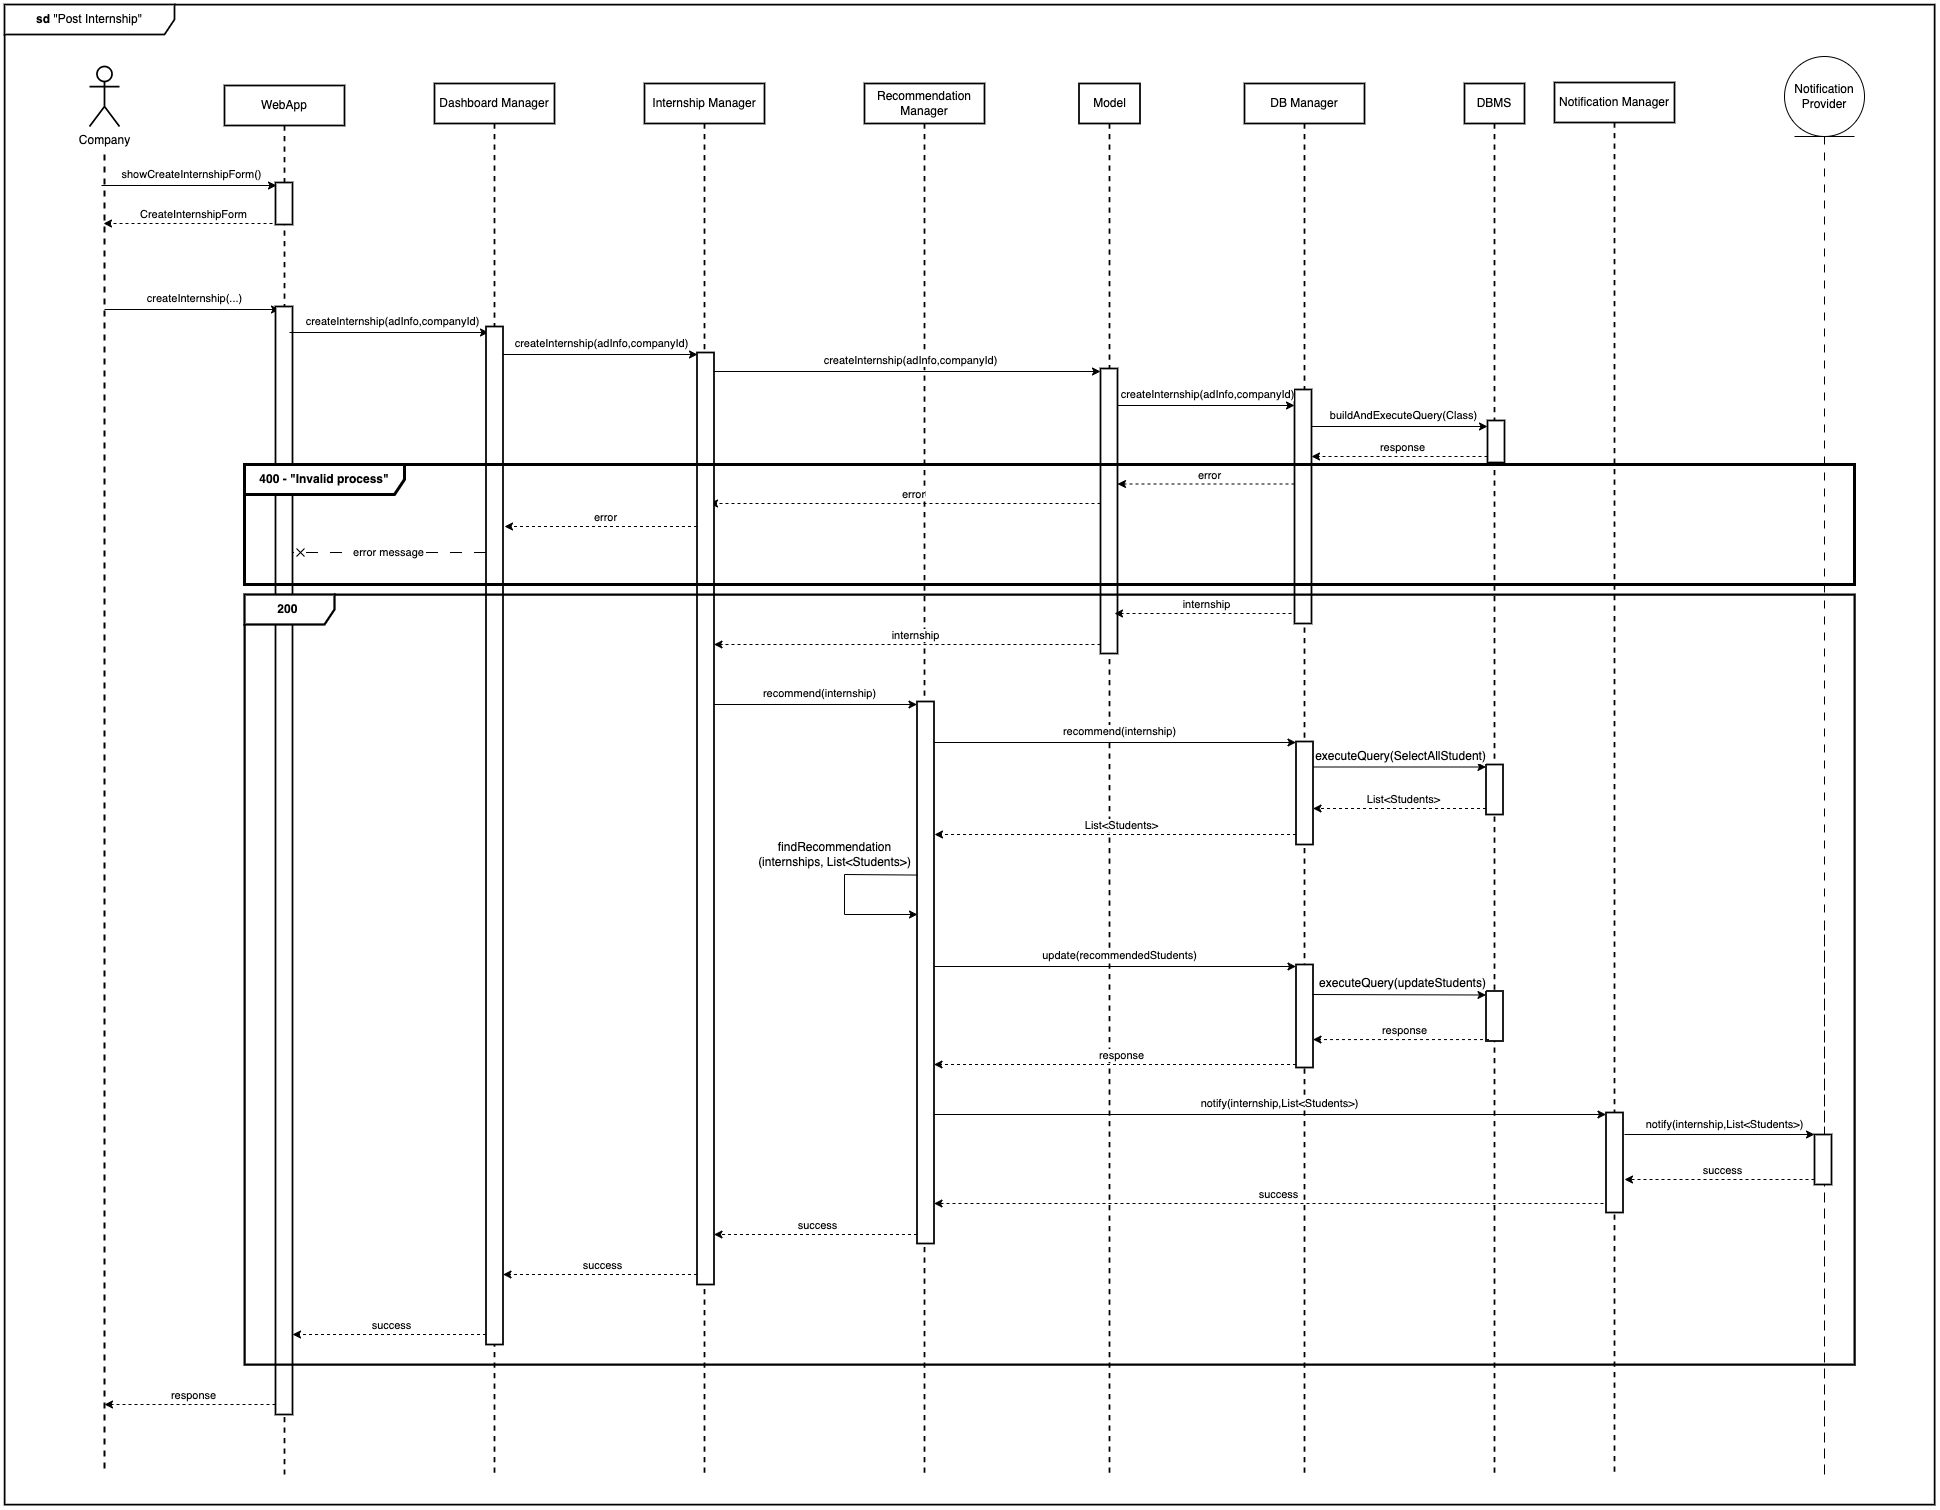
\includegraphics[scale = 0.25]{DD_figures/SingleDiagrams/postInternship.drawio.png}
    \caption{Company Create Internship}
    \centering
\end{figure}

\subsection{Component Interfaces}
\subsubsection{API Endpoints}
\subsection{Selected Architectural Styles and Patterns}
\subsection{Other Design Decisions}
\subsubsection{Scale-out}
\subsubsection{Relational Database}
\subsubsection{Token-Based Authentication and Authorization}
\subsubsection{Distributed MVC Pattern}

\section{User Interface Design}

\section{Requirements Traceability}

\section{Implementation, Integration and Testing Plan}
\subsection{Development Process and Approach}
\subsection{Implementation \& Integration Plan}
\subsubsection{Server Side}
\subsubsection{Client Side}
\subsubsection{Final Integration Test}
\subsection{Technologies}
\subsubsection{Development Technologies}
\subsubsection{Testing Technologies}

\section{Effort Spent}
\subsection{Effort Spent per Unit}

\section{References}
\subsection{References and Tools}

\end{document}
